\documentclass{exam}

\usepackage{siunitx} 
\usepackage{graphicx}
\usepackage[fleqn]{amsmath}
\usepackage{cancel}
\usepackage{float}
\usepackage{mdwlist}
\usepackage{booktabs}
\usepackage{cancel}
\usepackage{polynom}
\usepackage{caption}
\usepackage{fullpage}
\usepackage{comment}
\usepackage{enumerate}

\newcommand{\degree}{\ensuremath{^\circ}} 
\everymath{\displaystyle}

% \begin{figure}[H]
%   \centering
%   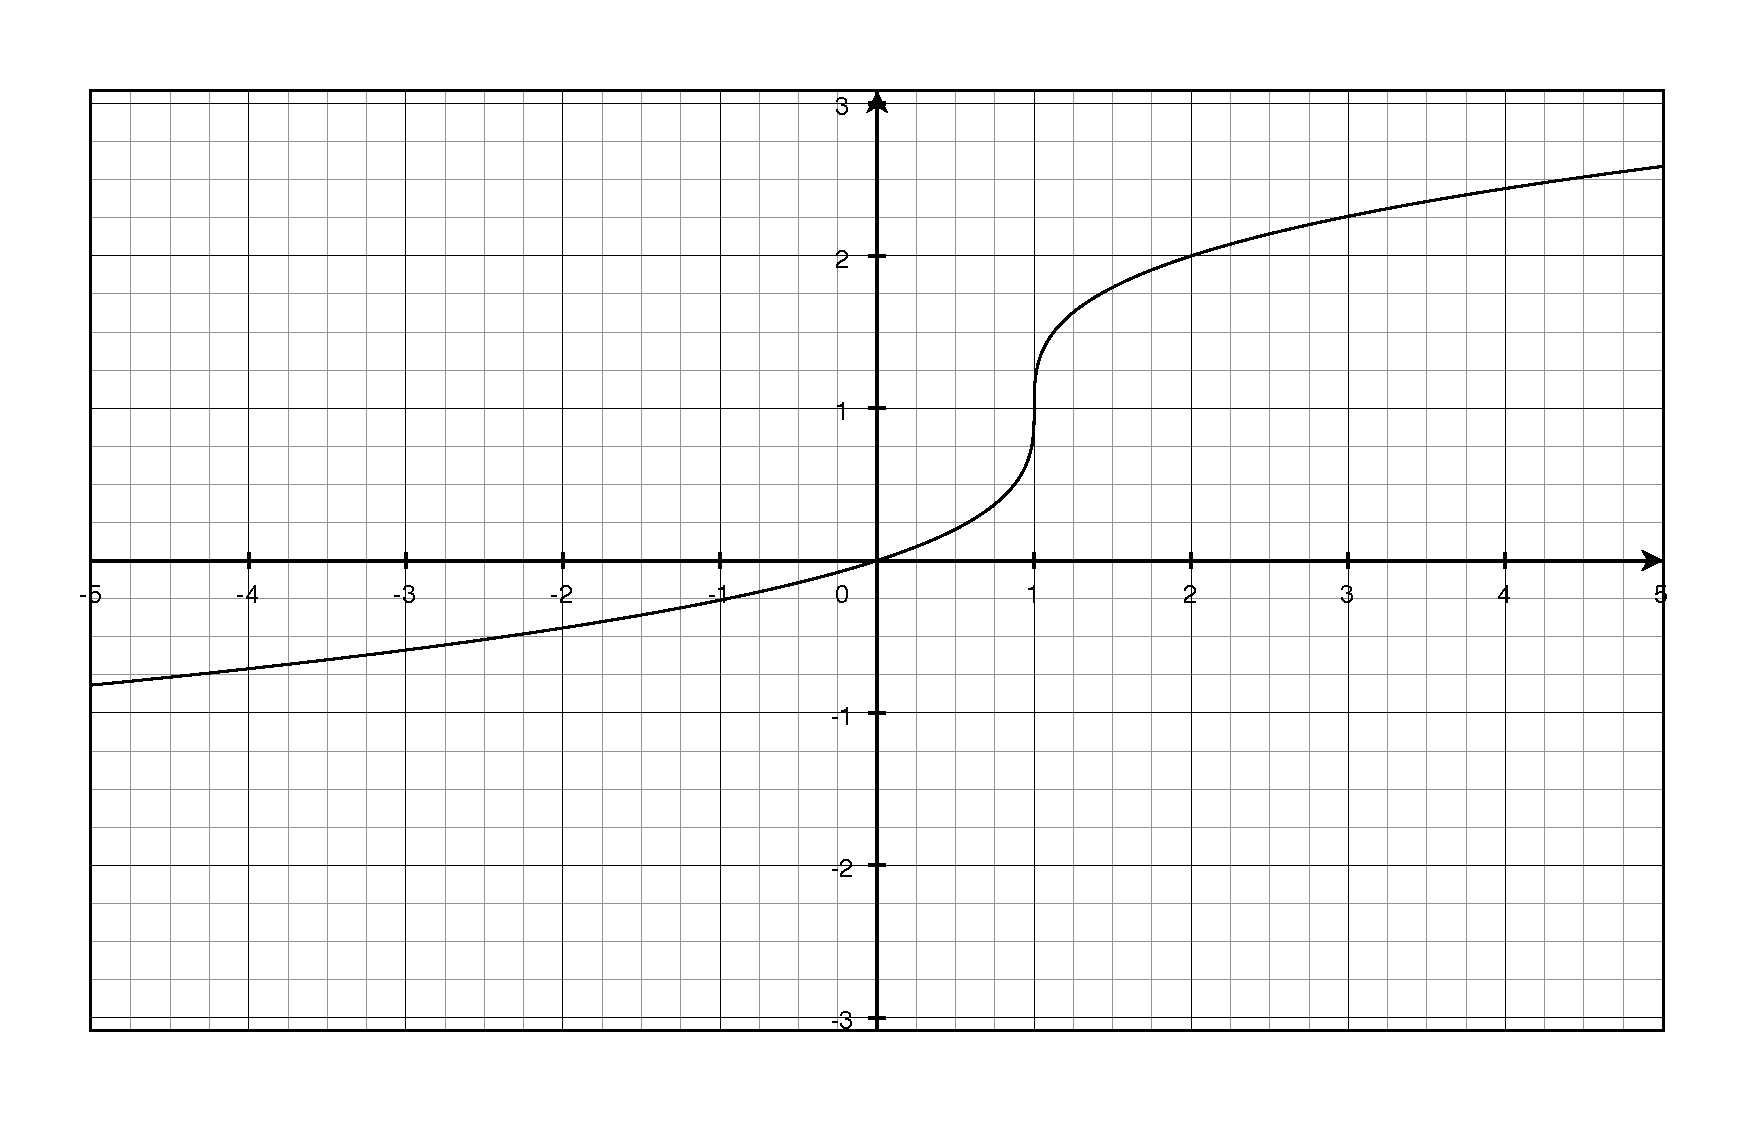
\includegraphics[scale=.3]{question7.eps}
%   \caption*{question 7}
% \end{figure}

% \begin{tabular}{cc}
%   \toprule
%   period & amplitude \\
%   \midrule
%     $\pi$ & $2$ \\
%   \bottomrule
% \end{tabular}

\printanswers
\excludecomment{comment}

\ifprintanswers 
  \usepackage{2in1, lscape} 
\fi

\author{}
\date{\today}
\title{Math 142 \\ Homework Two}

\begin{document}

  \maketitle

  \section{Homework}
  Section 5.2: 

  \section{Extra Credit}
  TO DO

  \ifprintanswers
    \section{Section 5.2}
    \begin{description}

      \item[1]
        \begin{tabular}[H]{rrr}
          \toprule
          $t$ & $\cos t$ & $\sin t$ \\
          \midrule
          $0$               & $1$                    & $0$ \\
          $\frac{\pi}{4}$   & $\frac{\sqrt{2}}{2}$   & $\frac{\sqrt{2}}{2}$ \\

          \midrule
          $\frac{\pi}{2}$   & $0$                    & $1$ \\
          $\frac{3 \pi}{4}$ & $- \frac{\sqrt{2}}{2}$ & $\frac{\sqrt{2}}{2}$ \\

          \midrule
          $\pi$             & $-1$                   & $0$ \\
          $\frac{5 \pi}{4}$ & $-\frac{\sqrt{2}}{2}$  & $-\frac{\sqrt{2}}{2}$ \\

          \midrule
          $\frac{3 \pi}{2}$ & $0$                    & $-1$ \\
          $\frac{7 \pi}{4}$ & $\frac{\sqrt{2}}{2}$   & $-\frac{\sqrt{2}}{2}$ \\

          \bottomrule
        \end{tabular}

      \item[2]
        \begin{tabular}[H]{rrr}
          \toprule
          $t$ & $\cos t$ & $\sin t$ \\

          \midrule
          $0$             & $1$                  & $0$ \\
          $\frac{\pi}{6}$ & $\frac{\sqrt{3}}{2}$ & $\frac{1}{2}$ \\
          $\frac{\pi}{3}$ & $\frac{1}{2}$        & $\frac{\sqrt{3}}{2}$   \\

          \midrule
          $\frac{\pi}{2}$   & $0$                   & $1$ \\
          $\frac{2\pi}{3}$  & $-\frac{1}{2}$        & $\frac{\sqrt{3}}{2}$   \\
          $\frac{5 \pi}{6}$ & $-\frac{\sqrt{3}}{2}$ & $\frac{1}{2}$ \\

          \midrule
          $\pi$             & $-1$                  & $0$ \\
          $\frac{7 \pi}{6}$ & $-\frac{\sqrt{3}}{2}$ & $-\frac{1}{2}$ \\
          $\frac{4 \pi}{3}$ & $-\frac{1}{2}$        & $-\frac{\sqrt{3}}{2}$   \\

          \midrule
          $\frac{3 \pi}{2}$  & $0$                  & $-1$ \\
          $\frac{5\pi}{3}$   & $\frac{1}{2}$        & $-\frac{\sqrt{3}}{2}$   \\
          $\frac{11 \pi}{6}$ & $\frac{\sqrt{3}}{2}$ & $-\frac{1}{2}$ \\

          \bottomrule
        \end{tabular}

      \item[3]
        \begin{align*}
          \sin \frac{2 \pi}{3} &= \frac{\sqrt{3}}{2} \\
          \cos \frac{2 \pi}{3} &= - \frac{1}{2} \\
          \tan \frac{2 \pi}{3} &= - \sqrt{3} \\
        \end{align*}

      \item[4]
        \begin{align*}
          \sin \frac{5 \pi}{6} &= \frac{1}{2} \\
          \cos \frac{5 \pi}{6} &= - \frac{\sqrt{3}}{2} \\
          \tan \frac{5 \pi}{6} &= - \frac{\sqrt{3}}{3} \\
        \end{align*}

      \item[5]
        \begin{align*}
          \sin \frac{7 \pi}{6}                 &= - \frac{1}{2} \\
          \sin \left( - \frac{\pi}{6} \right)  &= - \frac{1}{2} \\
          \sin \left( \frac{11 \pi}{6} \right) &= - \frac{1}{2} \\
        \end{align*}

      \item[6]
        \begin{align*}
          \cos \frac{5 \pi}{3}                  &= \frac{1}{2} \\
          \cos \left( - \frac{5 \pi}{3} \right) &= \frac{1}{2} \\
          \cos \frac{7 \pi}{3}                  &= \frac{1}{2} \\
        \end{align*}

      \item[7]
        \begin{align*}
          \cos \frac{3 \pi}{4} & = - \frac{\sqrt{2}}{2} \\
          \cos \frac{5 \pi}{4} & = - \frac{\sqrt{2}}{2} \\
          \cos \frac{7 \pi}{4} & = \frac{\sqrt{2}}{2} \\
        \end{align*}

      \item[8]
        \begin{align*}
          \sin \frac{3 \pi}{4} & = \frac{\sqrt{2}}{2} \\
          \sin \frac{5 \pi}{4} & = - \frac{\sqrt{2}}{2} \\
          \sin \frac{7 \pi}{4} & = - \frac{\sqrt{2}}{2} \\
        \end{align*}

      \item[9]
        \begin{align*}
          \sin \frac{7 \pi}{3} & = \frac{\sqrt{3}}{2} \\
          \csc \frac{7 \pi}{3} & = \frac{2 \sqrt{3}}{3} \\
          \cot \frac{7 \pi}{3} & = \frac{\sqrt{3}}{3} \\
        \end{align*}

      \item[10]
        \begin{align*}
          \cos \left( - \frac{\pi}{3} \right) & = \frac{1}{2} \\
          \sec \left( - \frac{\pi}{3} \right) & = 2 \\
          \tan \left( - \frac{\pi}{3} \right) & = - \sqrt{3} \\
        \end{align*}

      \item[11]
        \begin{align*}
          \sin \left( - \frac{\pi}{2} \right) & = -1 \\
          \cos \left( - \frac{\pi}{2} \right) & = 0 \\
          \cot \left( - \frac{\pi}{2} \right) & = 0 \\
        \end{align*}

      \item[12]
        \begin{align*}
          \sin \left( - \frac{3 \pi}{2} \right) & = 1 \\
          \cos \left( - \frac{3 \pi}{2} \right) & = 0 \\
          \cot \left( - \frac{3 \pi}{2} \right) & = 0 \\
        \end{align*}

      \item[13]
        \begin{align*}
          \sec \frac{11 \pi}{3}               & = 2 \\
          \csc \frac{11 \pi}{3}               & = - \frac{2 \sqrt{3}}{3} \\
          \sec \left( - \frac{\pi}{3} \right) & = 2 \\
        \end{align*}

      \item[14]
        \begin{align*}
          \cos \frac{7 \pi}{6} & = - \frac{\sqrt{3}}{2} \\
          \sec \frac{7 \pi}{6} & = - \frac{2 \sqrt{3}}{3} \\
          \csc \frac{7 \pi}{6} & = - 2 \\
        \end{align*}

      \item[15]
        \begin{align*}
          \tan \frac{5 \pi}{6}  & = - \frac{\sqrt{3}}{3} \\
          \tan \frac{7 \pi}{6}  & = \frac{\sqrt{3}}{3} \\
          \tan \frac{11 \pi}{6} & = - \frac{\sqrt{3}}{3} \\
        \end{align*}

      \item[16]
        \begin{align*}
          \cot \left( - \frac{\pi}{3} \right) & = - \frac{\sqrt{3}}{3} \\
          \cot \frac{2 \pi}{3}                & = - \frac{\sqrt{3}}{3} \\
          \cot \frac{5 \pi}{3}                & = - \frac{\sqrt{3}}{3} \\
        \end{align*}

      \item[17]
        \begin{align*}
          \cos \left( - \frac{\pi}{4} \right) & = \frac{\sqrt{2}}{2} \\
          \csc \left( - \frac{\pi}{4} \right) & = \sqrt{2} \\
          \cot \left( - \frac{\pi}{4} \right) & = 1 \\
        \end{align*}

      \item[18]
        \begin{align*}
          \sin \frac{5 \pi}{4} & = - \frac{\sqrt{2}}{2} \\
          \sec \frac{5 \pi}{4} & = - \sqrt{2} \\
          \tan \frac{5 \pi}{4} & = 1 \\
        \end{align*}

      \item[19]
        \begin{align*}
          \csc \left( - \frac{\pi}{2} \right) & = -1 \\
          \csc \frac{\pi}{2}                  & = 1 \\
          \csc \frac{3 \pi}{2}                & = - 1 \\
        \end{align*}

      \item[20]
        \begin{align*}
          \sec (- \pi) & = -1 \\
          \sec \pi     & = -1 \\
          \sec 4 \pi   & = 1 \\
        \end{align*}

      \item[21]
        \begin{align*}
          \sec 13 \pi & = -1 \\
          \cos 14 \pi & = 1 \\
          \tan 15 \pi & = 0 \\
        \end{align*}

      \item[22]
        \begin{align*}
          \sin \left( \frac{25 \pi}{2} \right) & = 1 \\
          \cos \left( \frac{25 \pi}{2} \right) & = 0 \\
          \cot \left( \frac{25 \pi}{2} \right) & = 0 \\
        \end{align*}

      \item[27]
        \begin{align*}
          \sin t & = \frac{4}{5} \\
          \cos t & = \frac{3}{5} \\
          \tan t & = \frac{4}{3} \\
        \end{align*}

      \item[28]
        \begin{align*}
          \sin t & = \frac{4}{5} \\
          \cos t & = - \frac{3}{5} \\
          \tan t & = - \frac{4}{3} \\
        \end{align*}

      \item[29]
        \begin{align*}
          \sin t & = - \frac{\sqrt{11}}{4} \\
          \cos t & = \frac{\sqrt{5}}{4} \\
          \tan t & = - \sqrt{\frac{11}{5}} \\
        \end{align*}

      \item[30]
        \begin{align*}
          \sin t & = - \frac{2 \sqrt{2}}{3} \\
          \cos t & = - \frac{1}{3} \\
          \tan t & = 2 \sqrt{2} \\
        \end{align*}

    \end{description}
  \else
    \vspace{1 cm}
    \begin{quote}
      \begin{em}
        TO DO
      \end{em}
    \end{quote}
    \hspace{1 cm} --Shunryu Suzuki
  \fi

\end{document}

